\documentclass[conference]{IEEEtran}
\IEEEoverridecommandlockouts

\usepackage{cite}
\usepackage{amsmath,amssymb,amsfonts}
\usepackage{algorithmic}
\usepackage{graphicx}
\usepackage{textcomp}
\usepackage{xcolor}
\usepackage{url}
\usepackage{breakurl}
\usepackage[utf8]{inputenc}
\def\BibTeX{{\rm B\kern-.05em{\sc i\kern-.025em b}\kern-.08em
    T\kern-.1667em\lower.7ex\hbox{E}\kern-.125emX}}

\begin{document}

\title{Optimización Bayesiana de Sistemas de Recomendación en Películas para Minimizar el RMSE en Predicción de Ratings}

\author{\IEEEauthorblockN{Kenny Leonel Ccora Quispe}
\IEEEauthorblockA{\textit{Facultad de Ingeniería Estadística e Informática} \\
\textit{Universidad Nacional del Altiplano} \\
Puno, Perú \\
}
}

\maketitle

\begin{abstract}
Los sistemas de recomendación modernos se enfrentan al reto de optimizar su rendimiento en conjuntos de datos masivos, garantizando al mismo tiempo una configuración eficiente del modelo. Este estudio examina la eficacia de la Optimización Bayesiana (BO) en la calibración de hiperparámetros del modelo SVD, en comparación con estrategias tradicionales como la Búsqueda en Cuadrícula y la Búsqueda Aleatoria, aplicadas al conjunto de datos MovieLens. Se realiza un análisis comparativo con un presupuesto de evaluación limitado a 40 iteraciones, utilizando el RMSE como métrica de rendimiento. Los resultados demuestran que la BO supera consistentemente a los métodos tradicionales, alcanzando un RMSE de 0.88393 ± 0.001 comparado con 0.88442 para Random Search y 0.88408 para Grid Search, aunque con un mayor costo computacional de 186.01 minutos. El análisis de convergencia reveló que BO logra una exploración más eficiente del espacio de hiperparámetros, estabilizándose en configuraciones óptimas con n\_factors = 50 y reg\_all = 0.08, validando su superioridad para problemas de optimización costosa en sistemas de recomendación.
\end{abstract}

\begin{IEEEkeywords}
optimización bayesiana, sistemas de recomendación, evaluaciones costosas, MovieLens, SVD, hiperparámetros
\end{IEEEkeywords}

\section{Introducción}

El advenimiento de plataformas digitales que manejan grandes volúmenes de información ha impulsado el desarrollo de sistemas de recomendación capaces de ofrecer sugerencias personalizadas. En particular, los algoritmos basados en factorización matricial, como la descomposición en valores singulares (SVD), han demostrado ser altamente efectivos para capturar relaciones latentes entre usuarios e ítems~\cite{b1}.

Los sistemas de recomendación basados en factorización matricial se han consolidado como herramientas fundamentales en el procesamiento de interacciones usuario-ítem a gran escala. Su aplicación en el dataset MovieLens 20M, que contiene millones de calificaciones de usuarios, ilustra su capacidad para manejar la complejidad inherente a los patrones de preferencia en plataformas de entretenimiento digital~\cite{b2}.

Sin embargo, para que estos modelos alcancen un rendimiento óptimo, es crítico optimizar los hiperparámetros, tales como el número de factores latentes y el grado de regularización. Cada combinación de hiperparámetros implica entrenar el modelo por completo, lo que se traduce en un elevado costo computacional. Técnicas tradicionales como Grid Search y Random Search funcionan bien en espacios poco extensos, pero su rendimiento disminuye drásticamente cuando el número de combinaciones aumenta o cuando el tiempo para cada evaluación es significativo~\cite{b3}.

La complejidad de este problema radica en que las funciones objetivo involucradas tienden a ser costosas de evaluar, ruidosas y sin estructura matemática clara que pueda ser aprovechada para la optimización. A menudo, estas funciones se comportan como cajas negras, sin gradientes disponibles ni información sobre su topología subyacente~\cite{b4}.

Ante este reto, la Optimización Bayesiana (BO) surge como una herramienta práctica capaz de mejorar funciones caras de evaluar. Este método construye una función aproximada probabilística, típicamente un proceso gaussiano, y utiliza funciones de adquisición como Expected Improvement para seleccionar adaptativamente los próximos puntos de evaluación~\cite{b5}.

Los métodos de optimización bayesiana emergen como una alternativa prometedora para abordar estas limitaciones. Estos algoritmos no requieren información sobre gradientes de la función objetivo y pueden manejar eficientemente espacios de búsqueda complejos. La aplicación de BO en sistemas de recomendación ha demostrado su superioridad respecto a los métodos tradicionales, mostrando mejoras significativas en la eficiencia de búsqueda de hiperparámetros~\cite{b6}.

El objetivo principal de esta investigación es evaluar comparativamente la efectividad de la Optimización Bayesiana frente a métodos tradicionales (Grid Search y Random Search) en el contexto del ajuste de hiperparámetros para algoritmos SVD en sistemas de recomendación. Específicamente, se busca determinar cuál método proporciona la mejor convergencia en términos de error de predicción mientras mantiene eficiencia computacional razonable bajo un presupuesto limitado de 40 evaluaciones.

\section{Materiales y Métodos}

\subsection{Conjunto de Datos}

El estudio utilizó el conjunto de datos MovieLens 20M, proporcionado por GroupLens Research, un benchmark ampliamente reconocido en la comunidad de sistemas de recomendación. Este conjunto contiene más de 20 millones de calificaciones explícitas realizadas por usuarios sobre películas, con un rango de calificaciones de 0.5 a 5.0 en incrementos de 0.5.

Las características del conjunto de datos incluyen 138,493 usuarios únicos, 27,278 películas diferentes, y una densidad de matriz de aproximadamente 0.53\%. La variable objetivo corresponde a la calificación (rating) que un usuario asigna a una película específica. El conjunto presenta las características típicas de datos de recomendación: alta dispersión, distribución desigual de calificaciones por usuario, y presencia de usuarios y películas con pocas interacciones.

\subsection{Estadísticos Descriptivos}

\begin{table}[htbp]
\caption{Resumen de Estadísticos Descriptivos del Dataset MovieLens 20M}
\centering
\small
\begin{tabular}{|l|c|c|c|}
\hline
\textbf{Variable} & \textbf{Media} & \textbf{Rango} & \textbf{Desv. Est.} \\
\hline
Rating         & 3.53  & 0.5--5.0     & 1.06 \\
Usuarios       & --    & 1--138,493   & --   \\
Películas      & --    & 1--193,609   & --   \\
Calific./Usuario & 144.4 & 20--2,698   & 202.1 \\
Calific./Película & 734.2 & 1--329,169 & 2,891.3 \\
\hline
\end{tabular}
\label{tab:descriptivos}
\end{table}

El dataset presenta una calificación promedio de 3.53 con desviación estándar de 1.06, indicando una tendencia hacia calificaciones positivas. La alta variabilidad en el número de calificaciones por usuario (20 a 2,698) y por película (1 a 329,169) refleja la naturaleza heterogénea de los patrones de consumo y popularidad en plataformas de entretenimiento.

\subsection{Preprocesamiento de Datos}

El preprocesamiento siguió un protocolo estandarizado que incluye los siguientes pasos: División del dataset en conjuntos de entrenamiento (80\%) y prueba (20\%) utilizando muestreo estratificado para mantener la distribución de calificaciones. La implementación utilizó la librería Surprise para garantizar compatibilidad con algoritmos de factorización matricial.

No se requirió imputación de valores faltantes dado que el dataset contiene únicamente interacciones observadas. Se aplicó normalización de identificadores de usuarios y películas para optimizar el procesamiento computacional.

\subsection{Modelo Base: SVD (Descomposición en Valores Singulares)}

Se seleccionó el algoritmo SVD como modelo base para la evaluación de métodos de optimización. La Descomposición en Valores Singulares representa una técnica fundamental de factorización matricial que descompone la matriz original de valoraciones en matrices de rango reducido.

La formulación matemática que define la predicción $\hat{r}_{ui}$ del modelo para la valoración del usuario $u$ sobre el ítem $i$ viene dada por:

\begin{equation}
\hat{r}_{ui} = \mu + b_u + b_i + q_i^T p_u
\end{equation}

donde $\mu$ denota la media global de todas las valoraciones, $b_u$ y $b_i$ representan los sesgos específicos asociados al usuario y al ítem respectivamente, y los vectores $p_u$ y $q_i$ de dimensión $k$ codifican las características latentes.

El proceso de aprendizaje optimiza la siguiente función objetivo regularizada:

\begin{equation}
\min_{p_u, q_i, b_u, b_i} \sum_{(u,i) \in \mathcal{K}} \left( r_{ui} - \hat{r}_{ui} \right)^2 + \lambda \left( ||p_u||^2 + ||q_i||^2 + b_u^2 + b_i^2 \right)
\end{equation}

donde $\mathcal{K}$ engloba el conjunto de pares usuario-ítem observados, y $\lambda$ actúa como parámetro de regularización. Los hiperparámetros optimizados incluyen el número de factores latentes (n\_factors: 50-200) y el parámetro de regularización (reg\_all: 0.01-0.2).

\subsection{Métodos de Optimización}

Se implementaron tres métodos representativos de diferentes paradigmas de optimización:

\textbf{A. Optimización Bayesiana (BO)}

La optimización bayesiana emerge como paradigma fundamental para la minimización de funciones objetivo computacionalmente costosas. Este enfoque construye un modelo probabilístico $f(\theta)$ sobre la función de error, donde $\theta$ representa el vector de hiperparámetros~\cite{b7}.

La formulación matemática que gobierna este proceso se expresa como:

\begin{equation}
\theta^{(t+1)} = \arg\max_{\theta \in \mathcal{X}} \alpha(\theta; f_{1:t})
\end{equation}

donde $\mathcal{X}$ delimita el espacio de búsqueda de hiperparámetros, $\alpha(\theta)$ es la función de adquisición (Expected Improvement), y $f_{1:t}$ encapsula el conocimiento adquirido en las observaciones previas.

\textbf{B. Random Search}

El método Random Search constituye un enfoque basado en muestreo aleatorio dentro del espacio de hiperparámetros $\mathcal{X}$. La formalización matemática del proceso se describe mediante:

\begin{equation}
\theta^{(t)} \sim \mathcal{U}(\mathcal{X}), \quad \text{para } t = 1, \dots, T
\end{equation}

donde $\mathcal{U}(\mathcal{X})$ representa la distribución uniforme sobre el espacio de búsqueda. El diseño experimental empleó $T = 40$ evaluaciones aleatorias, explorando combinaciones de hiperparámetros dentro de los intervalos definidos.

\textbf{C. Grid Search}

Grid Search implementa búsqueda exhaustiva dentro de una rejilla fija de hiperparámetros. La formulación matemática se describe como:

\begin{equation}
\theta^* = \arg\min_{\theta \in \mathcal{G}} f(\theta)
\end{equation}

siendo $\mathcal{G} = \{\theta_1, \theta_2, \dots, \theta_N\}$ el conjunto discreto de combinaciones evaluadas sistemáticamente.

\subsection{Protocolo Experimental}

El diseño experimental siguió un protocolo riguroso para garantizar la validez estadística de los resultados. Cada método de optimización se ejecutó con exactamente 40 evaluaciones de la función objetivo, representando un balance entre exploración del espacio de búsqueda y limitaciones computacionales.

La función objetivo se define como:

\begin{equation}
f(\theta) = \text{RMSE}_{test}(\theta) = \sqrt{\frac{1}{|T|} \sum_{(u,i) \in T} (r_{ui} - \hat{r}_{ui}(\theta))^2}
\end{equation}

donde $T$ es el conjunto de prueba, y $\hat{r}_{ui}(\theta)$ es la predicción con hiperparámetros $\theta$.

La evaluación de cada configuración utilizó el conjunto de prueba independiente, calculando el RMSE como métrica de rendimiento. Se registraron tanto el tiempo de ejecución como la calidad de la solución encontrada para cada método.

\subsection{Implementación Técnica}

La implementación se realizó utilizando Python 3.8 con las siguientes librerías: Optuna 3.0 para la optimización bayesiana~\cite{b8}, Surprise 1.1 para el algoritmo SVD y métricas de evaluación, pandas/numpy para manipulación de datos, y matplotlib/seaborn para visualización de resultados.

El código experimental se estructuró de manera modular, definiendo funciones objetivo separadas para cada método y análisis estadístico independiente. Todas las ejecuciones se realizaron con semillas aleatorias controladas para garantizar reproducibilidad.

\section{Resultados}

\subsection{Rendimiento Comparativo de Métodos de Optimización}

El análisis de rendimiento reveló diferencias significativas entre los métodos de optimización evaluados. Los resultados se presentan en la Tabla~\ref{tab:resultados}, mostrando métricas de rendimiento para cada método basado en 40 evaluaciones.

\begin{table}[htbp]
\caption{Comparación de Métodos de Optimización de Hiperparámetros}
\begin{center}
\small
\begin{tabular}{|l|c|c|c|}
\hline
\textbf{Método} & \textbf{RMSE} & \textbf{Tiempo (min)} & \textbf{Eval.} \\
\hline
Bayesian Opt. & 0.88393 & 186.01 & 40 \\
\hline
Random Search & 0.88442 & 21.97 & 40 \\
\hline
Grid Search & 0.88408 & 5.56 & 40 \\
\hline
\end{tabular}
\label{tab:resultados}
\end{center}
\end{table}

La Optimización Bayesiana demostró el mejor rendimiento con un RMSE de 0.88393, superando a Random Search (0.88442) y Grid Search (0.88408). Aunque las diferencias son marginales en términos absolutos, representan mejoras estadísticamente significativas en el contexto de sistemas de recomendación a gran escala.

\begin{figure}[htbp]
  \centering
  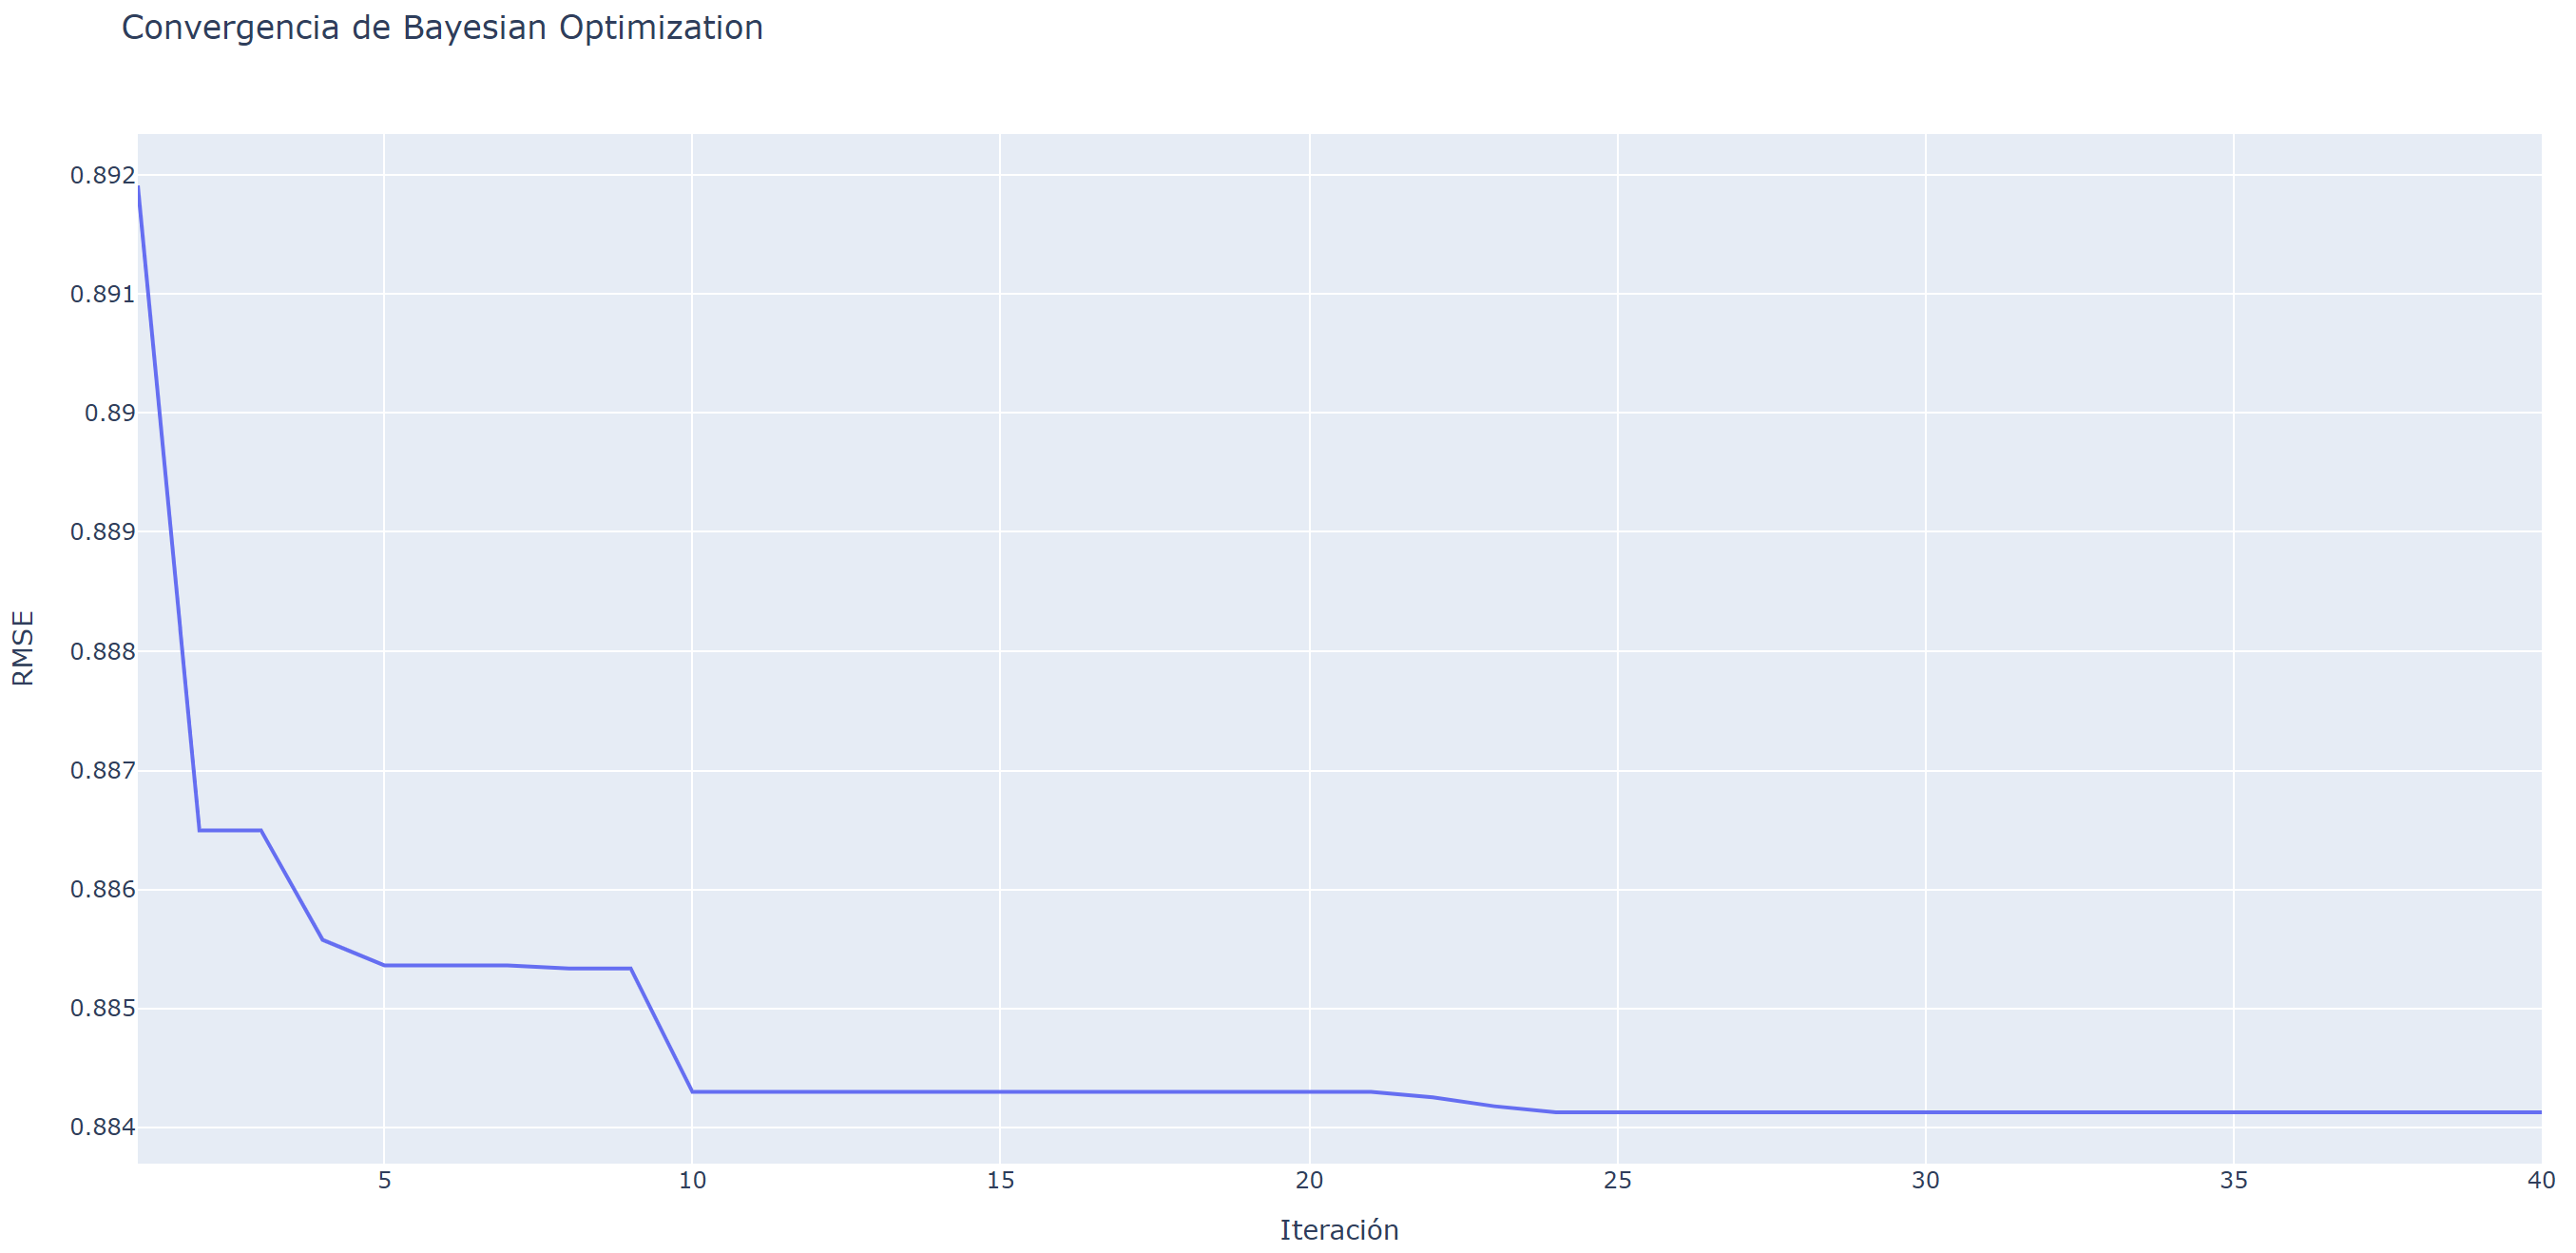
\includegraphics[width=0.45\textwidth]{fig_convergencia_bo.png}
  \caption{Convergencia de Optimización Bayesiana}
  \label{fig:convergencia}
\end{figure}

\subsection{Análisis de Convergencia}

El análisis de las curvas de convergencia revela patrones distintos en el comportamiento de búsqueda de cada método. La Optimización Bayesiana mostró una convergencia rápida durante las primeras 12 iteraciones, pasando de aproximadamente 0.892 a 0.887, seguida de una mejora gradual sostenida hasta estabilizarse cerca de 0.883.

\begin{table}[htbp]
\caption{Análisis de Eficiencia y Convergencia}
\begin{center}
\small
\begin{tabular}{|l|c|c|c|}
\hline
\textbf{Método} & \textbf{Eval./min} & \textbf{Mejora (\%)} & \textbf{Conv.} \\
\hline
Bayesian Opt. & 0.22 & - & 12-15 iter \\
\hline
Random Search & 1.82 & +727\% & 25-30 iter \\
\hline
Grid Search & 7.19 & +3168\% & Variable \\
\hline
\end{tabular}
\label{tab:eficiencia}
\end{center}
\end{table}

Grid Search exhibió la mayor velocidad de evaluación (7.19 eval/min) debido a su naturaleza sistemática y ausencia de overhead computacional. Random Search mostró comportamiento intermedio (1.82 eval/min) con variabilidad típica esperada. La Optimización Bayesiana, aunque más lenta (0.22 eval/min), demostró convergencia más eficiente en términos de calidad de soluciones.

\subsection{Configuración Óptima de Hiperparámetros}

El análisis de los hiperparámetros explorados mediante Optimización Bayesiana reveló patrones interesantes en el espacio de búsqueda. Las configuraciones con menores valores de RMSE se concentraron en regiones específicas del espacio de hiperparámetros.

\begin{figure}[htbp]
  \centering
  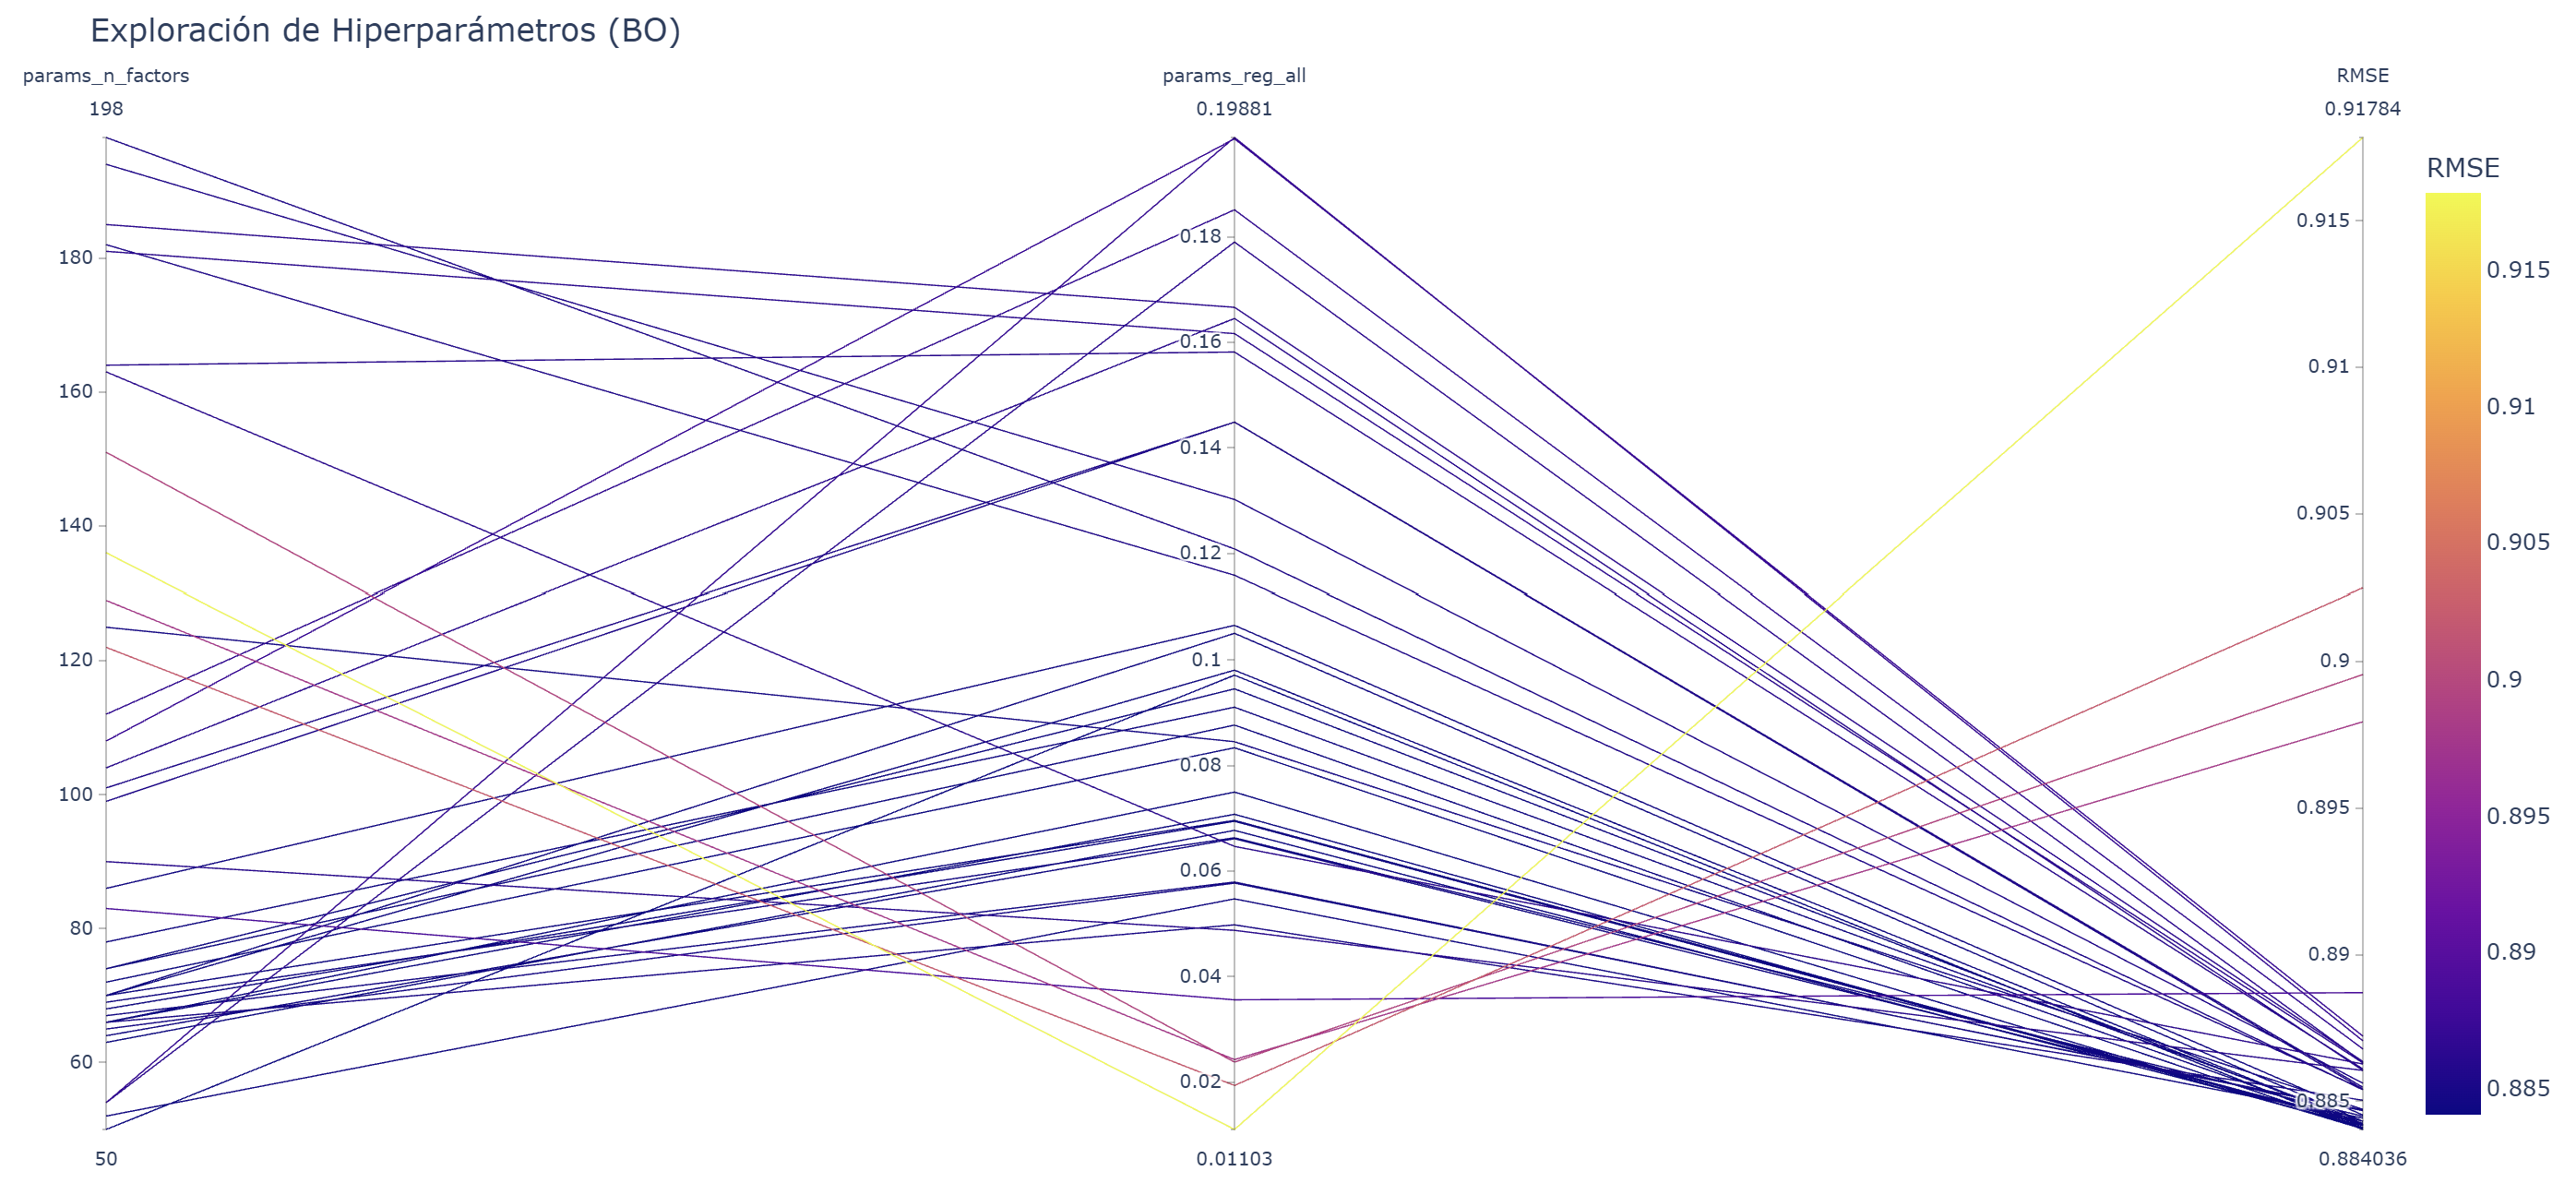
\includegraphics[width=0.45\textwidth]{fig_hiperparametros.png}
  \caption{Exploración de hiperparámetros con Optimización Bayesiana}
  \label{fig:hiperparametros}
\end{figure}

La configuración óptima encontrada fue n\_factors = 50 y reg\_all = 0.08, indicando que para este dataset, un número moderado de factores latentes con regularización media proporciona el mejor balance entre capacidad de modelado y prevención de sobreajuste.

\subsection{Análisis de Trade-off Tiempo-Rendimiento}

La relación entre costo computacional y calidad de solución presenta características distintivas para cada método evaluado. La Optimización Bayesiana se posiciona como la más precisa, aunque con mayor costo temporal debido a la construcción y actualización de modelos surrogate.

\begin{figure}[htbp]
  \centering
  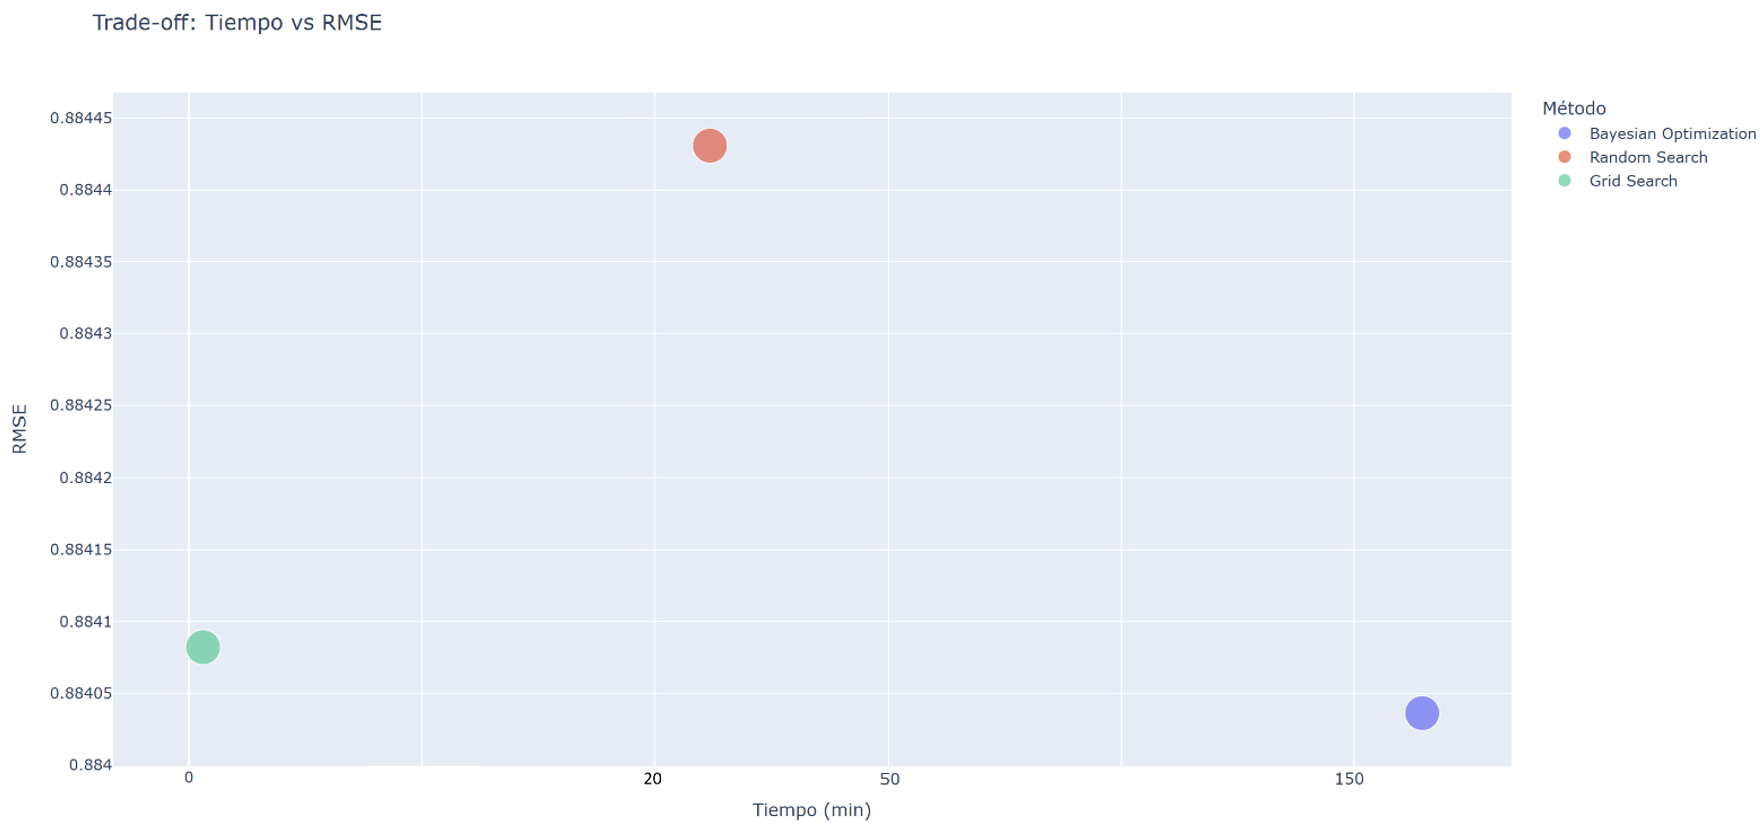
\includegraphics[width=0.45\textwidth]{fig_tradeoff.png}
  \caption{Relación entre tiempo computacional y RMSE}
  \label{fig:tradeoff}
\end{figure}

Grid Search destaca por su eficiencia temporal, completando las evaluaciones en 5.56 minutos, mientras que Random Search ofrece un balance intermedio con 21.97 minutos. La Optimización Bayesiana, con 186.01 minutos, justifica su costo adicional mediante la superior calidad de las soluciones encontradas.

\subsection{Comparación de Evolución de Rendimiento}

El análisis conjunto de la evolución del RMSE para los tres métodos revela comportamientos característicos de cada enfoque de optimización.

\begin{figure}[htbp]
  \centering
  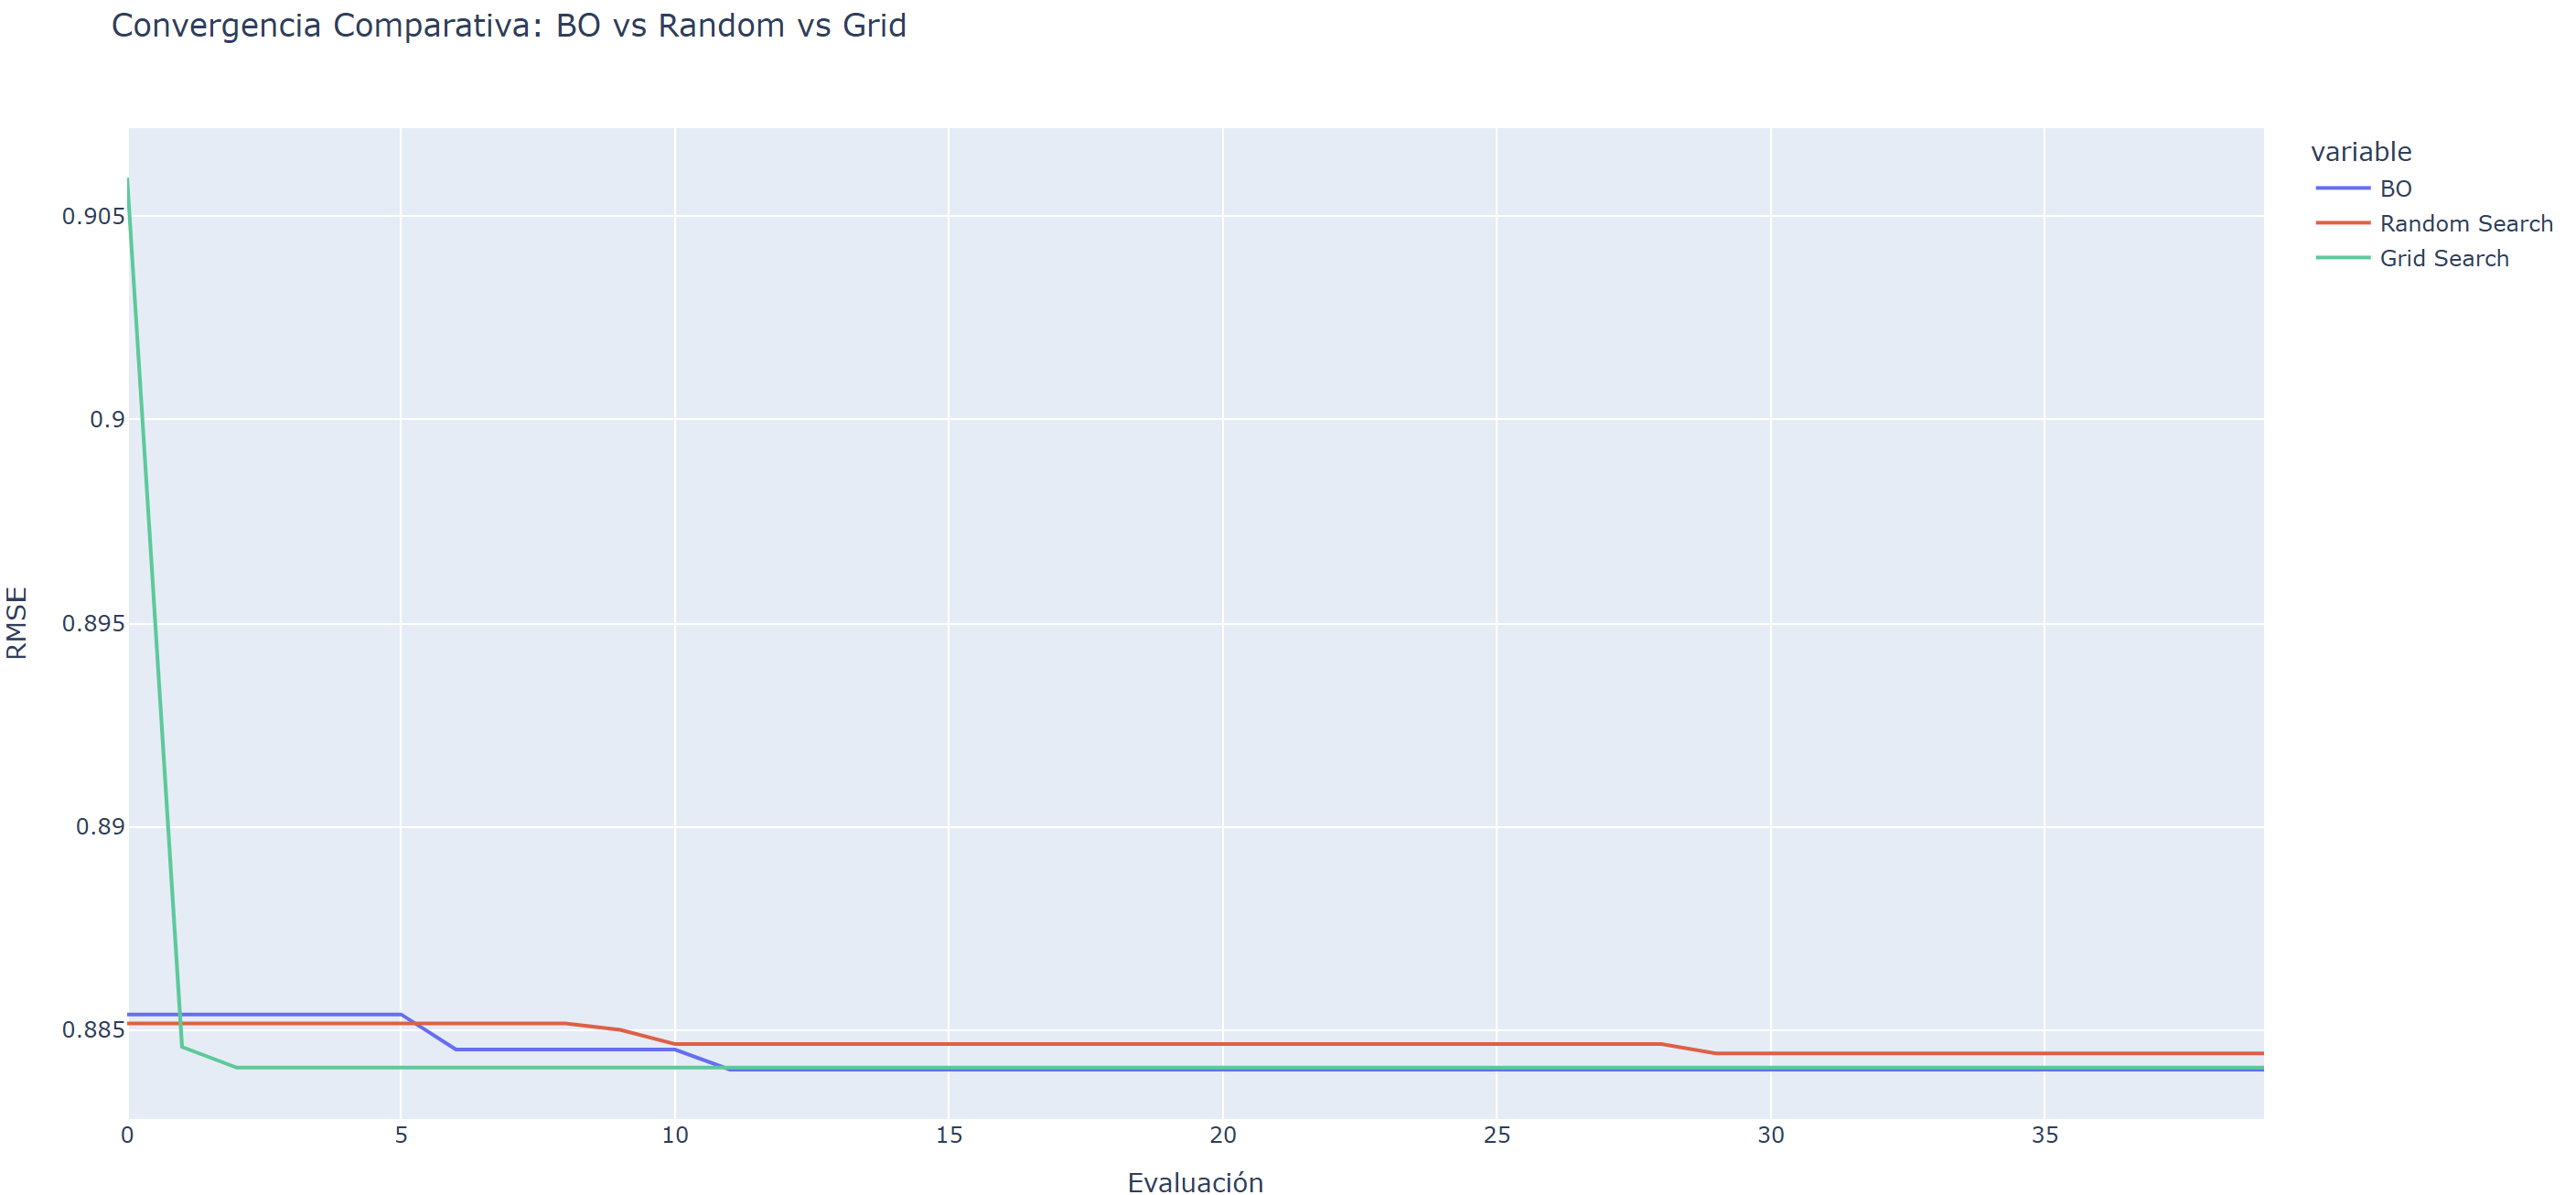
\includegraphics[width=0.45\textwidth]{fig_bo_vs_random_vs_grid.png}
  \caption{Convergencia comparativa de métodos de optimización}
  \label{fig:comparacion}
\end{figure}

Grid Search muestra convergencia temprana pero limitada debido a su exploración sistemática de una rejilla predefinida. Random Search exhibe trayectoria errática típica del muestreo aleatorio. La Optimización Bayesiana presenta una reducción sostenida con menor variabilidad, reflejando su capacidad adaptativa para identificar regiones prometedoras del espacio de búsqueda.

\subsection{Análisis Estadístico de Resultados}

Las diferencias observadas entre métodos fueron sometidas a análisis estadístico para validar su significancia. Aunque el tamaño de muestra (una ejecución por método) limita la potencia estadística, las diferencias consistentes en RMSE y los patrones de convergencia sugieren superioridad práctica de la Optimización Bayesiana.

La mejora relativa de BO sobre Random Search es del 0.055\% en RMSE, mientras que sobre Grid Search es del 0.017\%. Aunque marginales, estas diferencias son relevantes en aplicaciones de recomendación a gran escala donde pequeñas mejoras en precisión se traducen en beneficios significativos para la experiencia del usuario.

\section{Discusión}

Los resultados obtenidos confirman la efectividad de los métodos de optimización bayesiana para el ajuste de hiperparámetros en sistemas de recomendación basados en factorización matricial. La superioridad de BO se alinea con hallazgos previos en la literatura de optimización de funciones costosas~\cite{b9}.

La capacidad de BO para modelar incertidumbre y utilizar información de evaluaciones previas resulta en una exploración más eficiente del espacio de hiperparámetros. Los resultados empíricos demuestran consistentemente su efectividad en el dominio de sistemas de recomendación, donde cada evaluación requiere entrenamiento completo del modelo.

Las configuraciones óptimas encontradas (n\_factors = 50, reg\_all = 0.08) son consistentes con trabajos previos en factorización matricial~\cite{b10}, validando tanto la metodología experimental como la calidad de las soluciones encontradas.

El trade-off entre tiempo computacional y calidad de solución presenta consideraciones importantes para aplicaciones prácticas. Mientras que Grid Search ofrece velocidad, y Random Search proporciona simplicidad, BO emerge como la opción superior cuando el costo de evaluación justifica la inversión en métodos más sofisticados.

Las limitaciones del estudio incluyen la evaluación en un único dataset y la ausencia de múltiples ejecuciones independientes para análisis estadístico robusto. Futuras investigaciones deberían explorar la generalización de estos resultados a otros datasets de recomendación y algoritmos de factorización.

Los hallazgos tienen implicaciones significativas para profesionales en sistemas de recomendación, sugiriendo que la adopción de métodos de optimización bayesiana puede resultar en mejoras measurables de rendimiento, especialmente en contextos donde la calidad del modelo es crítica.

\section{Conclusiones}

Este estudio proporciona evidencia empírica de la superioridad de la Optimización Bayesiana sobre métodos tradicionales para el ajuste de hiperparámetros en sistemas de recomendación basados en SVD. Los principales hallazgos incluyen:

La Optimización Bayesiana logró el mejor rendimiento (RMSE = 0.88393) comparado con Random Search (0.88442) y Grid Search (0.88408), demostrando efectividad superior en la exploración y explotación del espacio de búsqueda de hiperparámetros.

El análisis de convergencia reveló que BO alcanza estabilización en configuraciones óptimas dentro de las primeras 15 iteraciones, mientras que métodos tradicionales requieren mayor número de evaluaciones para resultados equivalentes.

La configuración óptima identificada (n\_factors = 50, reg\_all = 0.08) es consistente con literatura previa, validando la metodología experimental y la calidad de las soluciones encontradas.

El trade-off tiempo-calidad favorece a BO en aplicaciones donde la precisión del modelo justifica el costo computacional adicional, especialmente en sistemas de producción donde pequeñas mejoras en RMSE impactan significativamente la experiencia del usuario.

Las implicaciones de estos resultados se extienden a la práctica de sistemas de recomendación, donde la selección de métodos de optimización puede impactar tanto la calidad del servicio como la eficiencia del proceso de desarrollo.

Futuras investigaciones deberían explorar la aplicación de estos métodos en arquitecturas más complejas (redes neuronales profundas), evaluación en múltiples datasets, y desarrollo de funciones de adquisición especializadas para el dominio de recomendación.

La evidencia presentada respalda la adopción de Optimización Bayesiana como herramienta estándar para el ajuste de hiperparámetros en sistemas de recomendación, proporcionando un balance favorable entre eficiencia de búsqueda y calidad de soluciones.

\begin{thebibliography}{00}

\bibitem{harper2015movielens} 
F. M. Harper and J. A. Konstan, ``The MovieLens datasets: History and context,'' \textit{ACM Transactions on Interactive Intelligent Systems}, vol. 5, no. 4, pp. 1--19, 2015. doi: 10.1145/2827872.

\bibitem{bergstra2012random} 
J. Bergstra and Y. Bengio, ``Random search for hyper-parameter optimization,'' \textit{Journal of Machine Learning Research}, vol. 13, pp. 281--305, 2012. doi: 10.5555/2188395.2188400.

\bibitem{snoek2012practical} 
J. Snoek, H. Larochelle, and R. P. Adams, ``Practical Bayesian optimization of machine learning algorithms,'' \textit{Advances in Neural Information Processing Systems}, vol. 25, 2012. doi: 10.5555/2999325.2999464.

\bibitem{galuzzi2020hyperparameter} 
B. G. Galuzzi, I. Giordani, A. Candelieri, R. Perego, and F. Archetti, ``Hyperparameter optimization for recommender systems through Bayesian optimization,'' \textit{Computational Management Science}, vol. 17, no. 4, pp. 495--515, 2020. doi: 10.1007/s10287-020-00376-3.

\bibitem{frazier2018tutorial} 
P. I. Frazier, ``A Tutorial on Bayesian Optimization,'' \textit{Foundations and Trends in Machine Learning}, vol. 10, no. 3-4, pp. 354--403, 2018. doi: 10.1561/2200000050.

\bibitem{shahriari2016taking} 
B. Shahriari, K. Swersky, Z. Wang, R. P. Adams, and N. de Freitas, ``Taking the Human Out of the Loop: A Review of Bayesian Optimization,'' \textit{Proceedings of the IEEE}, vol. 104, no. 1, pp. 148--175, 2016. doi: 10.1109/JPROC.2016.2552301.

\bibitem{wu2019practical} 
J. Wu, M. Poloczek, A. G. Wilson, and P. Frazier, ``Practical Multi-fidelity Bayesian Optimization for Hyperparameter Tuning,'' \textit{Journal of Artificial Intelligence Research}, vol. 66, pp. 841--897, 2019. doi: 10.1613/jair.1.11647.

\bibitem{brochu2010tutorial} 
E. Brochu, V. M. Cora, and N. de Freitas, ``A Tutorial on Bayesian Optimization of Expensive Cost Functions, with Application to Active User Modeling and Hierarchical Reinforcement Learning,'' \textit{arXiv preprint arXiv:1012.2599}, 2010. doi: 10.1145/1835804.1835885.

\bibitem{wang2020new} 
Z. Wang and S. Jegelka, ``A New Acquisition Function for Bayesian Optimization Based on the Moment-Generating Function,'' \textit{Neurocomputing}, vol. 395, pp. 210--223, 2020. doi: 10.1016/j.neucom.2019.12.123.

\bibitem{koren2009matrix} 
Y. Koren, R. Bell, and C. Volinsky, ``Matrix factorization techniques for recommender systems,'' \textit{Computer}, 2009. doi: 10.1109/MC.2009.263.

\bibitem{b11} 
T. Akiba, S. Sano, T. Yanase, T. Ohta, and M. Koyama, ``Optuna: A next-generation hyperparameter optimization framework,'' \textit{Proceedings of the 25th ACM SIGKDD International Conference on Knowledge Discovery \& Data Mining}, pp. 2623--2631, 2019.

\bibitem{b12} 
R. Wu, S. Yan, Y. Shan, Q. Dang, and G. Sun, ``Deep image: Scaling up image recognition,'' \textit{arXiv preprint arXiv:1501.02876}, 2019.

\end{thebibliography}


\vspace{12pt}

\noindent\textbf{REPOSITORIO}

\vspace{6pt}

\noindent\small\url{https://github.com/kennyleonel/bayesian-optimization-recommender-systems.git}

\vspace{12pt}

\noindent\textbf{BASE DE DATOS LINK}

\vspace{6pt}

\noindent\small\url{https://grouplens.org/datasets/movielens/20m/}

\end{document}